% GNUPLOT: LaTeX picture with Postscript
\begingroup
  \makeatletter
  \providecommand\color[2][]{%
    \GenericError{(gnuplot) \space\space\space\@spaces}{%
      Package color not loaded in conjunction with
      terminal option `colourtext'%
    }{See the gnuplot documentation for explanation.%
    }{Either use 'blacktext' in gnuplot or load the package
      color.sty in LaTeX.}%
    \renewcommand\color[2][]{}%
  }%
  \providecommand\includegraphics[2][]{%
    \GenericError{(gnuplot) \space\space\space\@spaces}{%
      Package graphicx or graphics not loaded%
    }{See the gnuplot documentation for explanation.%
    }{The gnuplot epslatex terminal needs graphicx.sty or graphics.sty.}%
    \renewcommand\includegraphics[2][]{}%
  }%
  \providecommand\rotatebox[2]{#2}%
  \@ifundefined{ifGPcolor}{%
    \newif\ifGPcolor
    \GPcolortrue
  }{}%
  \@ifundefined{ifGPblacktext}{%
    \newif\ifGPblacktext
    \GPblacktextfalse
  }{}%
  % define a \g@addto@macro without @ in the name:
  \let\gplgaddtomacro\g@addto@macro
  % define empty templates for all commands taking text:
  \gdef\gplbacktext{}%
  \gdef\gplfronttext{}%
  \makeatother
  \ifGPblacktext
    % no textcolor at all
    \def\colorrgb#1{}%
    \def\colorgray#1{}%
  \else
    % gray or color?
    \ifGPcolor
      \def\colorrgb#1{\color[rgb]{#1}}%
      \def\colorgray#1{\color[gray]{#1}}%
      \expandafter\def\csname LTw\endcsname{\color{white}}%
      \expandafter\def\csname LTb\endcsname{\color{black}}%
      \expandafter\def\csname LTa\endcsname{\color{black}}%
      \expandafter\def\csname LT0\endcsname{\color[rgb]{1,0,0}}%
      \expandafter\def\csname LT1\endcsname{\color[rgb]{0,1,0}}%
      \expandafter\def\csname LT2\endcsname{\color[rgb]{0,0,1}}%
      \expandafter\def\csname LT3\endcsname{\color[rgb]{1,0,1}}%
      \expandafter\def\csname LT4\endcsname{\color[rgb]{0,1,1}}%
      \expandafter\def\csname LT5\endcsname{\color[rgb]{1,1,0}}%
      \expandafter\def\csname LT6\endcsname{\color[rgb]{0,0,0}}%
      \expandafter\def\csname LT7\endcsname{\color[rgb]{1,0.3,0}}%
      \expandafter\def\csname LT8\endcsname{\color[rgb]{0.5,0.5,0.5}}%
    \else
      % gray
      \def\colorrgb#1{\color{black}}%
      \def\colorgray#1{\color[gray]{#1}}%
      \expandafter\def\csname LTw\endcsname{\color{white}}%
      \expandafter\def\csname LTb\endcsname{\color{black}}%
      \expandafter\def\csname LTa\endcsname{\color{black}}%
      \expandafter\def\csname LT0\endcsname{\color{black}}%
      \expandafter\def\csname LT1\endcsname{\color{black}}%
      \expandafter\def\csname LT2\endcsname{\color{black}}%
      \expandafter\def\csname LT3\endcsname{\color{black}}%
      \expandafter\def\csname LT4\endcsname{\color{black}}%
      \expandafter\def\csname LT5\endcsname{\color{black}}%
      \expandafter\def\csname LT6\endcsname{\color{black}}%
      \expandafter\def\csname LT7\endcsname{\color{black}}%
      \expandafter\def\csname LT8\endcsname{\color{black}}%
    \fi
  \fi
    \setlength{\unitlength}{0.0500bp}%
    \ifx\gptboxheight\undefined%
      \newlength{\gptboxheight}%
      \newlength{\gptboxwidth}%
      \newsavebox{\gptboxtext}%
    \fi%
    \setlength{\fboxrule}{0.5pt}%
    \setlength{\fboxsep}{1pt}%
\begin{picture}(7360.00,5660.00)%
    \gplgaddtomacro\gplbacktext{%
      \csname LTb\endcsname%%
      \put(537,3326){\makebox(0,0)[r]{\strut{}$1$}}%
      \csname LTb\endcsname%%
      \put(537,3722){\makebox(0,0)[r]{\strut{}$1.2$}}%
      \csname LTb\endcsname%%
      \put(537,4118){\makebox(0,0)[r]{\strut{}$1.4$}}%
      \csname LTb\endcsname%%
      \put(537,4514){\makebox(0,0)[r]{\strut{}$1.6$}}%
      \csname LTb\endcsname%%
      \put(537,4910){\makebox(0,0)[r]{\strut{}$1.8$}}%
      \csname LTb\endcsname%%
      \put(537,5306){\makebox(0,0)[r]{\strut{}$2$}}%
      \csname LTb\endcsname%%
      \put(622,3171){\makebox(0,0){\strut{}$1$}}%
      \csname LTb\endcsname%%
      \put(1131,3171){\makebox(0,0){\strut{}$1.2$}}%
      \csname LTb\endcsname%%
      \put(1641,3171){\makebox(0,0){\strut{}$1.4$}}%
      \csname LTb\endcsname%%
      \put(2150,3171){\makebox(0,0){\strut{}$1.6$}}%
      \csname LTb\endcsname%%
      \put(2660,3171){\makebox(0,0){\strut{}$1.8$}}%
      \csname LTb\endcsname%%
      \put(3169,3171){\makebox(0,0){\strut{}$2$}}%
      \csname LTb\endcsname%%
      \put(902,5177){\makebox(0,0)[l]{\strut{}(a)}}%
    }%
    \gplgaddtomacro\gplfronttext{%
      \csname LTb\endcsname%%
      \put(42,4415){\rotatebox{-270}{\makebox(0,0){\strut{}\footnotesize MOF-FF bond lengths ($\AA$)}}}%
      \csname LTb\endcsname%%
      \put(2023,2939){\makebox(0,0){\strut{}\footnotesize DFT bond lengths ($\AA$)}}%
      \csname LTb\endcsname%%
      \put(3136,4065){\makebox(0,0)[r]{\strut{}\ZIFCH3}}%
      \csname LTb\endcsname%%
      \put(3136,3802){\makebox(0,0)[r]{\strut{}\ZIFCl}}%
      \csname LTb\endcsname%%
      \put(3136,3539){\makebox(0,0)[r]{\strut{}\ZIFBr}}%
    }%
    \gplgaddtomacro\gplbacktext{%
      \csname LTb\endcsname%%
      \put(4217,3326){\makebox(0,0)[r]{\strut{}$100$}}%
      \csname LTb\endcsname%%
      \put(4217,3871){\makebox(0,0)[r]{\strut{}$110$}}%
      \csname LTb\endcsname%%
      \put(4217,4415){\makebox(0,0)[r]{\strut{}$120$}}%
      \csname LTb\endcsname%%
      \put(4217,4960){\makebox(0,0)[r]{\strut{}$130$}}%
      \csname LTb\endcsname%%
      \put(4217,5504){\makebox(0,0)[r]{\strut{}$140$}}%
      \csname LTb\endcsname%%
      \put(4302,3171){\makebox(0,0){\strut{}$100$}}%
      \csname LTb\endcsname%%
      \put(5003,3171){\makebox(0,0){\strut{}$110$}}%
      \csname LTb\endcsname%%
      \put(5703,3171){\makebox(0,0){\strut{}$120$}}%
      \csname LTb\endcsname%%
      \put(6404,3171){\makebox(0,0){\strut{}$130$}}%
      \csname LTb\endcsname%%
      \put(7104,3171){\makebox(0,0){\strut{}$140$}}%
      \csname LTb\endcsname%%
      \put(4582,5177){\makebox(0,0)[l]{\strut{}(b)}}%
    }%
    \gplgaddtomacro\gplfronttext{%
      \csname LTb\endcsname%%
      \put(3722,4415){\rotatebox{-270}{\makebox(0,0){\strut{}\footnotesize MOF-FF angles (°)}}}%
      \csname LTb\endcsname%%
      \put(5703,2939){\makebox(0,0){\strut{}\footnotesize DFT angles (°)}}%
    }%
    \gplgaddtomacro\gplbacktext{%
      \csname LTb\endcsname%%
      \put(622,496){\makebox(0,0)[r]{\strut{}$-200$}}%
      \csname LTb\endcsname%%
      \put(622,1041){\makebox(0,0)[r]{\strut{}$-100$}}%
      \csname LTb\endcsname%%
      \put(622,1586){\makebox(0,0)[r]{\strut{}$0$}}%
      \csname LTb\endcsname%%
      \put(622,2130){\makebox(0,0)[r]{\strut{}$100$}}%
      \csname LTb\endcsname%%
      \put(622,2675){\makebox(0,0)[r]{\strut{}$200$}}%
      \csname LTb\endcsname%%
      \put(707,341){\makebox(0,0){\strut{}$-200$}}%
      \csname LTb\endcsname%%
      \put(1386,341){\makebox(0,0){\strut{}$-100$}}%
      \csname LTb\endcsname%%
      \put(2066,341){\makebox(0,0){\strut{}$0$}}%
      \csname LTb\endcsname%%
      \put(2745,341){\makebox(0,0){\strut{}$100$}}%
      \csname LTb\endcsname%%
      \put(3424,341){\makebox(0,0){\strut{}$200$}}%
      \csname LTb\endcsname%%
      \put(979,2348){\makebox(0,0)[l]{\strut{}(c)}}%
    }%
    \gplgaddtomacro\gplfronttext{%
      \csname LTb\endcsname%%
      \put(42,1585){\rotatebox{-270}{\makebox(0,0){\strut{}\footnotesize MOF-FF dihedral angles (°)}}}%
      \csname LTb\endcsname%%
      \put(2065,109){\makebox(0,0){\strut{}\footnotesize DFT dihedral angles (°)}}%
    }%
    \gplgaddtomacro\gplbacktext{%
      \csname LTb\endcsname%%
      \put(4302,496){\makebox(0,0)[r]{\strut{}$0$}}%
      \csname LTb\endcsname%%
      \put(4302,1041){\makebox(0,0)[r]{\strut{}$500$}}%
      \csname LTb\endcsname%%
      \put(4302,1586){\makebox(0,0)[r]{\strut{}$1000$}}%
      \csname LTb\endcsname%%
      \put(4302,2130){\makebox(0,0)[r]{\strut{}$1500$}}%
      \csname LTb\endcsname%%
      \put(4302,2675){\makebox(0,0)[r]{\strut{}$2000$}}%
      \csname LTb\endcsname%%
      \put(4387,341){\makebox(0,0){\strut{}$0$}}%
      \csname LTb\endcsname%%
      \put(5066,341){\makebox(0,0){\strut{}$500$}}%
      \csname LTb\endcsname%%
      \put(5746,341){\makebox(0,0){\strut{}$1000$}}%
      \csname LTb\endcsname%%
      \put(6425,341){\makebox(0,0){\strut{}$1500$}}%
      \csname LTb\endcsname%%
      \put(7104,341){\makebox(0,0){\strut{}$2000$}}%
      \csname LTb\endcsname%%
      \put(4659,2348){\makebox(0,0)[l]{\strut{}(d)}}%
    }%
    \gplgaddtomacro\gplfronttext{%
      \csname LTb\endcsname%%
      \put(3722,1585){\rotatebox{-270}{\makebox(0,0){\strut{}\footnotesize MOF-FF vibrations (\si{cm^{-1}})}}}%
      \csname LTb\endcsname%%
      \put(5745,109){\makebox(0,0){\strut{}\footnotesize DFT vibrations (\si{cm^{-1}})}}%
    }%
    \gplbacktext
    \put(0,0){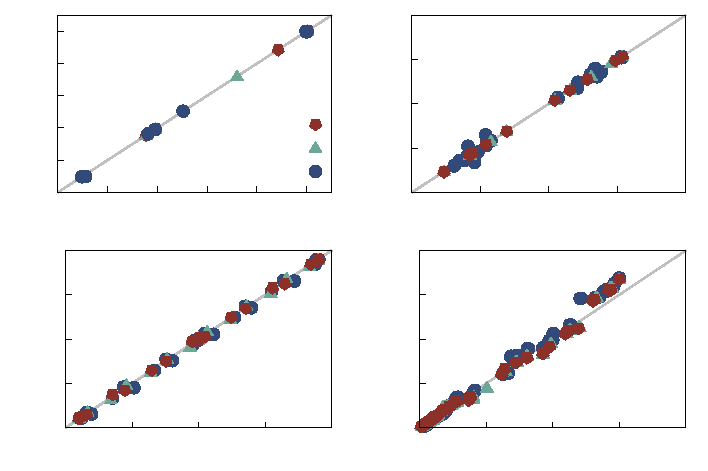
\includegraphics{mof-ff-validation}}%
    \gplfronttext
  \end{picture}%
\endgroup
